\documentclass{beamer}

\usepackage{dirtytalk}
\usepackage{hyperref}
\usepackage{listings}
\usepackage{color}
\definecolor{atomPurple}{RGB}{198,120,221}
\definecolor{atomRed}{RGB}{203,15,64}
\definecolor{atomGreen}{RGB}{0,128,0}
\definecolor{atomGreyLight}{RGB}{171,178,191}
\definecolor{atomGreyDark}{RGB}{92,99,112}
\definecolor{atomBlack}{RGB}{56,58,66}

\lstset{
language=C,
numbers=left,
showstringspaces=false,
tabsize=4,
columns=flexible,
keepspaces=true,
keywordstyle=\color{atomRed},
stringstyle=\color{atomGreen},
commentstyle=\color{atomGreyDark}
}

\title{Increasing Relevance of Rank by Price}
\author{Vaughan Kitchen}
\date{July 9, 2019}

\begin{document}

\begin{frame}
\titlepage
\end{frame}

\begin{frame}{What is IR?}
	\say{
\textbf{Information retrieval (IR)} is the activity of obtaining information system resources that are relevant to an information need from a collection of those resources. Searches can be based on full-text or other content-based indexing. Information retrieval is the science of searching for information in a document, searching for documents themselves, and also searching for the metadata that describes data, and for databases of texts, images or sounds.
	}
	\rightline{{\rm --- wikipedia}}

	(fulfilling a users information needs)

\end{frame}

\begin{frame}{eCommerce Search}
	A search engine integrated into an online store helping users find products. Users perform queries where the search engine tries to match keywords to products that it has stored. Can have a deeper semantic understanding of text, do query rewriting, or fuzzy matching which seperates it from a database (which just does look ups).
\end{frame}

\begin{frame}{The Problem with eCommerce Search}
	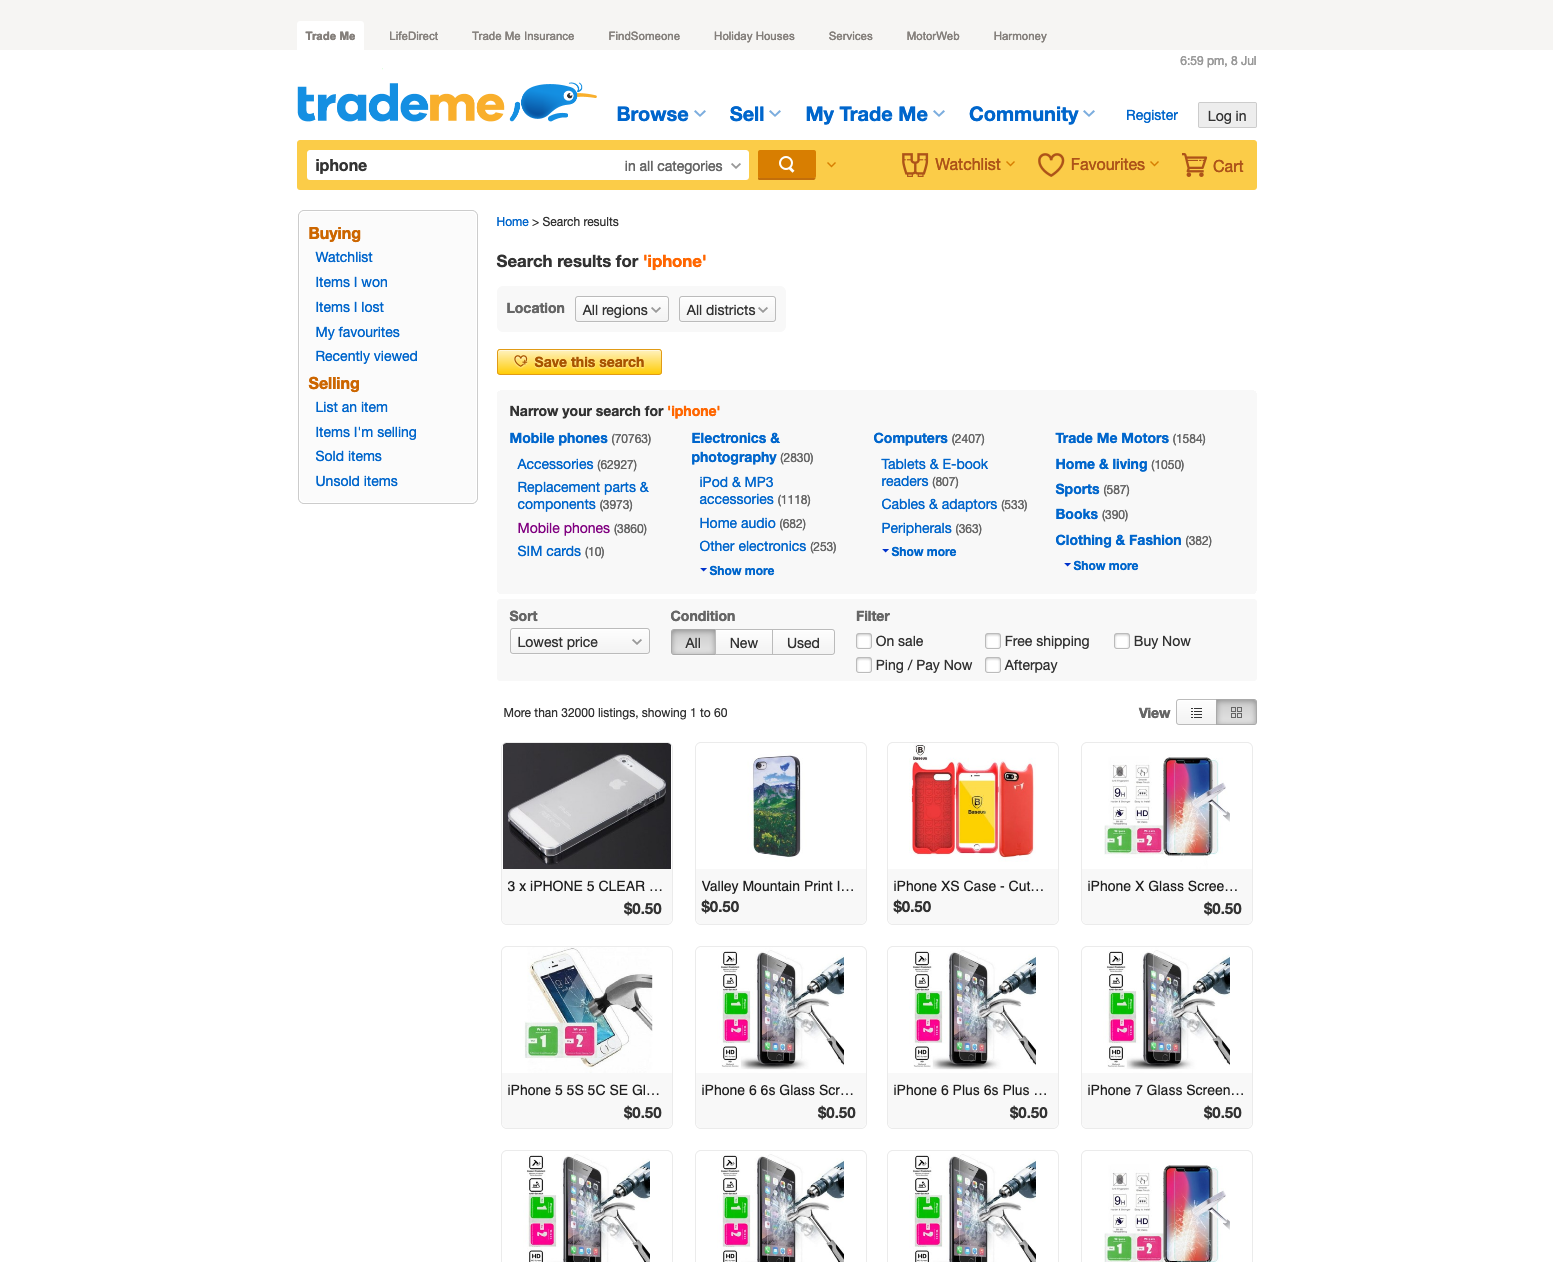
\includegraphics[width=\linewidth]{trademe-iphone.png}
\end{frame}

\begin{frame}{The Problem with eCommerce Search}
	\begin{itemize}
		\item These are not iPhones
		\item Many of the results are not relevant
		\item Often the non-relevant results are cheaper
		\item Non-relevant results feature as the top results
	\end{itemize}
\end{frame}

\begin{frame}{Some Definitions}
	\say{
\textbf{recall} (also known as sensitivity) is the fraction of relevant instances that have been retrieved over the total amount of relevant instances
	}
	\rightline{{\rm --- wikipedia}}
	\say{
\textbf{precision} (also called positive predictive value) is the fraction of relevant instances among the retrieved instances
	}
	\rightline{{\rm --- wikipedia}}
	\begin{itemize}
		\item Recall = Found/Total No. Relevant
		\item Precision = Found/Total Returned
		\item Often seen as Precision at n, P@n, e.g. P@10
	\end{itemize}
\end{frame}

\begin{frame}{Precision or Recall?}
	\begin{itemize}
		\item P@10 result poor when price ordered
		\item High precision needed
		\item User always wants cheapest item
		\item Will use competitor if they're cheaper
		\item High recall needed
		\item High accuracy needed
	\end{itemize}
\end{frame}

\begin{frame}{Metrics}
	\begin{itemize}
		\item P@n: Precision at n
		\item Mean Average Precision (MAP): Sum(P-at-reldoc-n) / Relevant, averaged
		\item Discounted Cumulative Gain: Relevance gain of extra documents discounted for index in list
		\item Normalized Discounted Cumulative Gain: DCG normalized against ideal result
		\item (Collaboration with eBay and IR community)
	\end{itemize}
\end{frame}

\begin{frame}{SIGIR Data Challenge 2019}
	\begin{itemize}
		\item High Accuracy Recall Task
		\item Opened May 27
		\item Closes July 18
		\item Three phases: Unsupervised, Supervised, Combined
		\item Approximately 900,000 documents with price, title, category
		\item 150 Queries
		\item Binary classification
	\end{itemize}
\end{frame}

\begin{frame}{SIGIR Data Challenge 2019}
	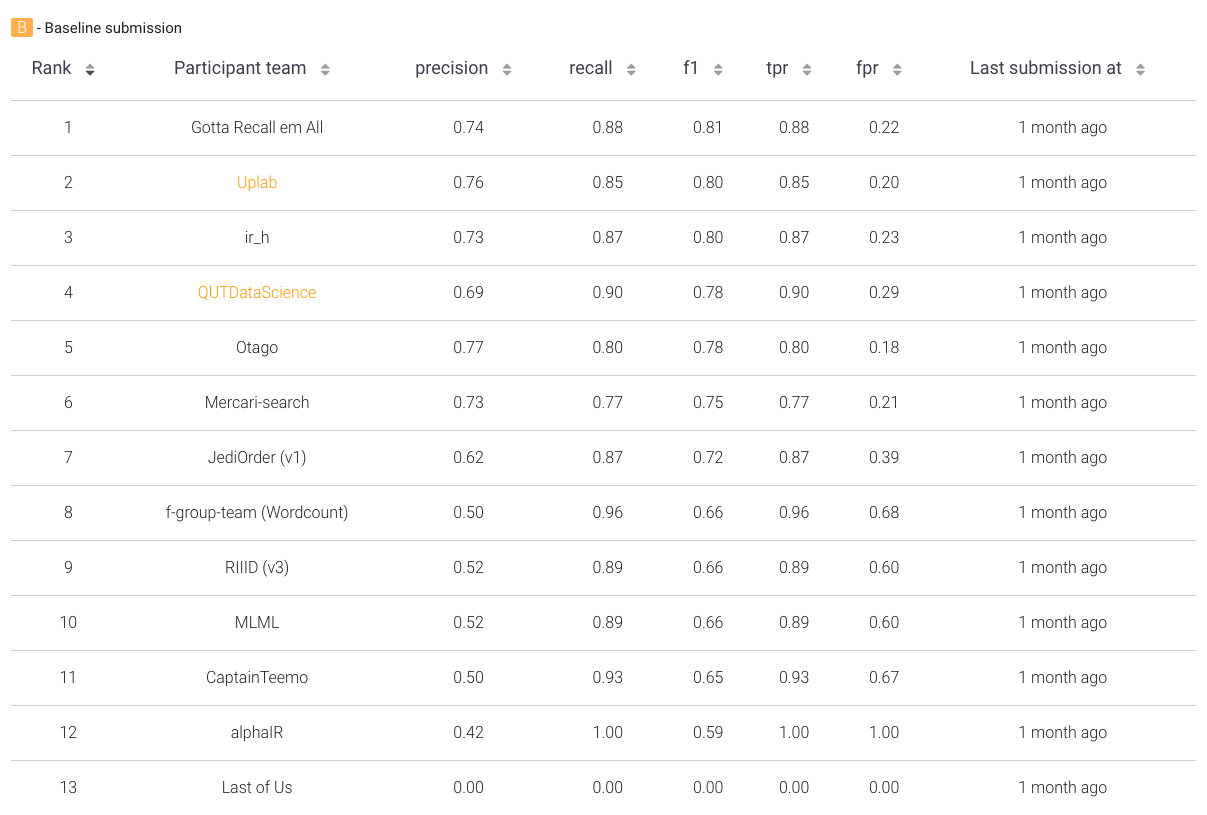
\includegraphics[width=\linewidth]{data-challenge.png}
\end{frame}

\begin{frame}{SIGIR Data Challenge 2019}
	\begin{itemize}
		\item 5th/12 successful submissions in Unsupervised phase
		\item Unable to submit in supervised phase due to busyness
		\item Attempting final phase over next two weeks
		\item Search engine written from scratch
		\item Conjunctive search with Porter's stemming
		\item Final attempt will be with Entity Linking
	\end{itemize}
\end{frame}

\begin{frame}{spaCy Named Entity Recognition}
	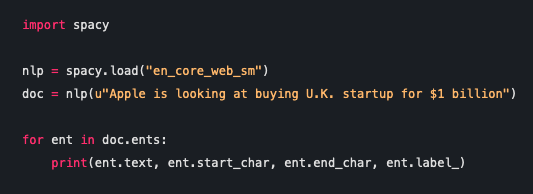
\includegraphics[width=\linewidth]{spacy-code.png}
\end{frame}

\begin{frame}{spaCy Named Entity Recognition}
	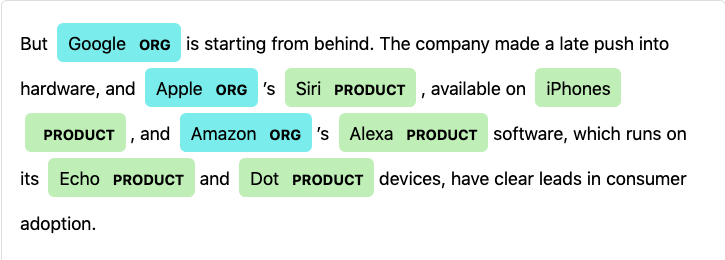
\includegraphics[width=\linewidth]{spacy-result.png}
\end{frame}

\begin{frame}{Entity Linking}
	Fast and Space-Efficient Entity Linking in Queries (Blanco et al.)
	\begin{itemize}
		\item Fast and Space-Efficient Entity Linking in Queries (Blanco et al.)
		\item Hash table to entities with thesaurus mined from query logs weighted to preferred results
		\item Successful for query segmentation
		\item ``clinton falls asleep" $\rightarrow$ ``clinton falls $\vert$ asleep", ``clinton $\vert$ falls asleep"
	\end{itemize}
	A Multi-View-Based Collective Entity Linking Method (Liu et al.)
	\begin{itemize}
		\item Collective Entity Linking
		\item Considers \textit{description, background knowledge, references} and \textit{entity graph structure}
		\item \textit{description} gives best performance to complexity ratio
	\end{itemize}
\end{frame}

\begin{frame}{Entity Linking}
	\begin{itemize}
		\item Requires large scale preprocessing of Wikipedia
		\item Performance considerations in practice
		\item Unsure on overall effect on result quality
		\item Short text (titles only) may affect results
	\end{itemize}
\end{frame}

\begin{frame}{References}
	\begin{itemize}
		\item Roi Blanco, Giuseppe Ottaviano, and Edgar Meij. 2015. Fast and Space-Efficient Entity Linking in Queries. Proceedings of the Eigth ACM International Conference on Web Search and Data Mining, Pages 179-188. http://dx.doi.org/10.1145/2684822.2685317
		\item Ming Liu, Gu Gong, Bing Qin, and Ting Liu. 2019. A Multi-View–Based Collective Entity Linking Method. ACM Transactions on Information Systems 37, 2, Article 23 (Feb.2019),29pages. https://doi.org/10.1145/3300197
	\end{itemize}
\end{frame}

\begin{frame}{Questions?}
\end{frame}

\end{document}
